\chapter{Methodology}
Our method can be seen as an approach built upon the idea of leaf-root path or sub-path (section~\ref{leafrootmethod}), in an operation tree~\cite{goodsurvey}.

Analogously,

\section{Intuitions}
Operators with semantic implication of commutative property (e.g. addition and multiplication) are exhaustively used in mathematical language. The ability to identify the identical equations for any permutation is very essential for a mathematical similarity search engine. 
Given this as a start point, the leaf-root paths have the advantage to cope this so that we do not need to generate different order of patterns to match formulae with commutative operator. 
To illustrate this, we know leaf-root paths from an operation tree (see figure~\ref{oprtreeExample}) is generated through traversing in a bottom-up (or top-down) fashion from a tree, thus path string is independent with the relative position of operands from same father node.

Breakdown
These properties Avoid information augmentation on index as some other structure-based methods do (e.g. all sub-terms of an expression are indexed in MWS) therefore it help save storage space.


\begin{figure}
\begin{minipage}[b]{2.65in}
\begin{center}
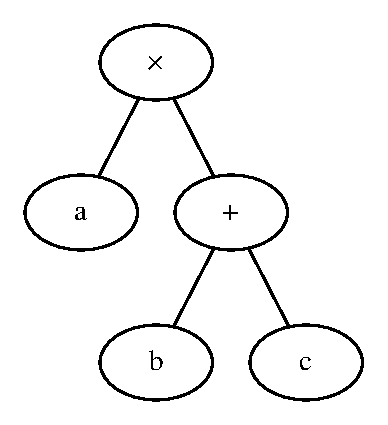
\includegraphics[height=1.8in]{leafroottree}
\\$a(b+c)$ in operation tree
\end{center}
\end{minipage}
\hspace*{.38in}
\begin{minipage}[b]{2.65in}
\begin{center}
\raisebox{.0in}{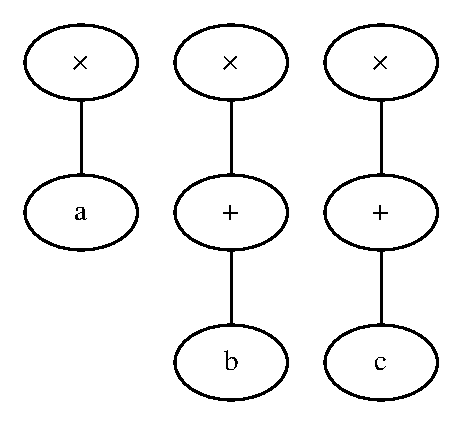
\includegraphics[height=1.8in]{leafrootpath}}
Generated leaf-root paths
\end{center}
\end{minipage}
\caption{Leaf-Root Path Example}\label{oprtreeExample}
\end{figure}

\section{Formal Description}
The basic ideas used in our approach, to test whether a mathematical expression is an sub-structure of another, to prune and to constrain search process are the foundation work in our method. It is desired to give a description in a formal language so that we can deliver these ideas in the most precise way. Some important observations as well as brief justifications are provided after definitions.

\subsection{Definitions}

\subsubsection{Formula tree}
Formula tree is an labeled rooted tree $T = T(V,E,r)$ with root $r$, where each vertex $v \in V(T)$ is associated with a label $\ell(v) \in \mathbf{R}$ mapped by function $\ell$, and each leaf $l \in V(T)$ is also associated with a symbol $s(v) \in \mathbf{R}$ mapped by function $s$.

\subsubsection{Formula subtree}
Given formula tree $S$ and $T$, we say $S$ is a forumla subtree of $T$ if there exists an injective mapping $\phi: V(S) \rightarrow V(T)$ satisfying:

\begin{enumerate}
\item 
$\forall\; (v_1,v_2) \in E(S)$, we have $(f(v_1),f(v_2)) \in E(T)$;
\item
$\forall\; v \in V(S)$, we have $\ell(v) = \ell(\phi(v))$;
\item
Every leaf in $S$ is also a leaf in $T$.
\end{enumerate}
Such a mapping $\phi$ is called a formula subtree isomorphlic embedding (or formula embedding) for $S \rightarrow T$. 
If satisfied, we denote $S \preceq_l T$ on $\Phi$, where $\Phi$ ($\Phi \neq \emptyset$) is the set of all the possible formula embeddings for $S \rightarrow T$.

\subsection{Observations}
\subsubsection*{Observation \#1} 
For two formula trees which satisfiy $T_q \preceq_l T_d$ on $\Phi$, then $\forall\; \phi \in \Phi,\, p \in g(T_q)$, also any vertex $v$ along path $p$, the following properties are obtained:
\begin{eqnarray}
\deg(v) \le \deg(\phi(v)) \label{equ1} \\
\left| p \right| = \left| \phi(p) \right| \label{equ2} \\
\ell(p) = \ell(\phi(p)) \label{equ3} \\
\left| g(T_q) \right| \le \left| g(T_d) \right| \label{equ4}
\end{eqnarray}

\subsubsection*{Observation \#2} 
Given two formula trees $T_q$ and $T_d$, if $\left| g(T_q) \right| = 1$ and $\ell(g(T_{q})) \subseteq \ell(g(T_d))$, then $T_q \preceq_l T_d$.

\subsubsection*{Observation \#3} 
For two formula trees $T_q$ and $T_d$, if $T_q = T(V,E,r) \preceq_l T_d$ on $\Phi$,  
$\forall a,b \in g(T_q)$ and a mapping $\phi \in \Phi$. 
Let $T_d' = \, ^{t}T_d$ where $t = \phi(r)$ and $a' = \phi(a) \in g(T_d')$, $b' \in g(T_d')$ then:
$$
\begin{array}{lcr}
b' = \phi(b)  & \Rightarrow & 
\left| \mathrm{lcp}(a,b) \right| = \left| \mathrm{lcp}(a',b') \right|
\end{array}
$$
Furthermore, $\forall\; c \in g(T_q)\; s.t.\; \left| \mathrm{lcp}(a,b) \right| \neq \left| \mathrm{lcp}(a,c) \right| $, we have
$$
\begin{array}{lcr}
\left| \mathrm{lcp}(a,b) \right| = \left| \mathrm{lcp}(a',b') \right|
& \Rightarrow &
b' \neq \phi(c)
\end{array} 
$$

\subsubsection*{Observation \#4} 
Given an index $\Pi$ and a formula tree $T_q$, $\forall\; T_d \in \Pi$:
If $T_q \preceq_l T_d$ on $\Phi$, then $\exists\; \hat{p} \in \mathbf{P},\; s.t.$
$$
T_d \in \bigcap_{p \in L} \mathcal{I}_{\Pi}(p)
$$
where $L = \ell(\hat{p} \cdot g(T_q))$.
